\documentclass{article}

\title{Progetto ``Collectors"}
\author{Daniele Borgna}

\date{5 luglio 2023}

% indice cliccabile
\usepackage{hyperref}
\hypersetup{hidelinks}

% per utilizzare includegraphics
\usepackage{graphicx}

% per impostare i margini più sottili
\usepackage[a4paper, margin=2cm]{geometry}

% per scrivere tra parentesi quadre
\usepackage{textcomp}

% per scrivere gli accenti
\usepackage[utf8]{inputenc}

% per riportare il codice
\usepackage{listings}
\usepackage{color}
\definecolor{dkgreen}{rgb}{0,0.6,0}
\definecolor{gray}{rgb}{0.5,0.5,0.5}
\definecolor{myorange}{RGB}{235, 134, 52}
\lstset{language=SQL,
  basicstyle={\small\ttfamily},
  belowskip=3mm,
  breakatwhitespace=true,
  breaklines=true,
  classoffset=0,
  columns=flexible,
  framexleftmargin=0.25em,
  frameshape={}{yy}{}{}, %To remove to vertical lines on left, set `frameshape={}{}{}{}`
  keywordstyle=\color{blue},
  otherkeywords={DECLARE, SIGNAL, FUNCTION, RETURN, RETURNS, REFERENCES, UNSIGNED, NEW, BY, DELIMITER, END, PROCEDURE, DATABASE, IF, USE, USER, BOOLEAN, IDENT, IFIED, TO, AU, _INCREMENT}, % Parole chiave personalizzate 
  numbers=left, %If you want line numbers, set `numbers=left`
  numberstyle=\tiny\color{gray},
  showstringspaces=false,
  stringstyle=\color{myorange},
  tabsize=3,
  xleftmargin =1em,
  commentstyle=\color{dkgreen}
}


\begin{document}
\maketitle

\pagebreak

\tableofcontents

\pagebreak

\section{Modello entità-relazione}
Di seguito il modello E-R con relative note a margine per concetti ed assunzioni non modellabili.
\begin{center}
    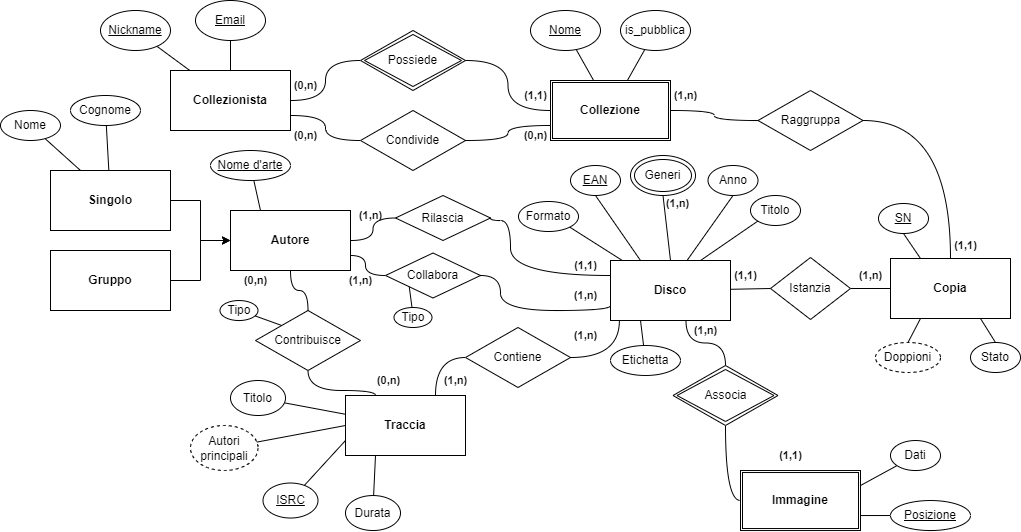
\includegraphics[width=\linewidth]{ER_ldb.png}
\end{center}

\subsection{Assunzioni}
\begin{enumerate}
    \item Ogni singola copia di un disco può appartenere ad esattamente una collezione. Ciò perché, essendo un sistema fortemente orientato alle collezioni, ritengo non sia utile caricare copie di dischi senza inserirle in alcuna collezione.
    \item Ogni disco può essere classificato in almeno un genere.
    \item Un disco è rilasciato da un solo artista (principale) ma possono esserci eventuali artisti secondari.
    \item Due dischi sono uguali se hanno stesso EAN (barcode). L'EAN è infatti uguale per due prodotti uguali, ma diverso se i prodotti sono diversi anche in un minimo particolare (es: versione deluxe del disco, cd oppure vinile, immagini diverse ...).
    \item Per distinguere invece copie dello \underline{stesso disco} (quindi stesso EAN) utilizziamo il Serial Number (SN): tali copie possono variare solo nello stato di conservazione, mentre formato, EAN, anno e tutti gli altri attributi devono essere identici.
    \item Uno stesso autore può contribuire a tracce diverse in modi diversi: ad esempio per una traccia può essere il produttore, mentre per un'altra può essere il cantante.
    \item Un gruppo è rappresentato solo da un nome d'arte, senza indicare nome e cognome dei singoli componenti. Assumo inoltre che non esistano autori (gruppi o singoli) con stesso nome d'arte.
    \item Il codice ISRC (international standard recording code) garantisce l'univocità di supporti audio e video musicali (fonte: fimi.it)
\end{enumerate}

\subsection{Note a margine}
\begin{enumerate}
    \item Come detto nell'assunzione 3, il "tipo" di contributo in una traccia (o disco) da parte di un autore può variare da traccia a traccia. Di conseguenza, l'attributo "Tipo" è legato alle relazioni "Contribuisce" e "Rilascia" e non all'autore.
    \item Il flag ``is\_pubblica" dell'entità "Collezione" indica, come facilmente intuibile, se una collezione è pubblica (ovvero visibile da chiunque) o meno. Nel caso in cui non fosse pubblica, si può distinguere ulteriormente in \textbf{condivisa}, se la lista dei collezionisti con cui è condivisa non è vuota, oppure \textbf{privata} se tale lista è vuota.
    \item L'entità "Disco" contiene le informazioni generali, mentre l'entità "Copia" si riferisce alla singola copia in possesso del collezionista.
    \item Nell'entità "Disco", l'attributo anno si riferisce all'anno di pubblicazione.
    \item L' "immagine" è identificata dal disco di cui fa parte e dalla posizione in cui è allocata. Non possono infatti esserci più immagini nella stessa posizione sullo stesso disco (qualsiasi copia di quel disco).
    \item L'attributo dati dell'entità "Immagine" consiste nel file contenente l'immagine.
    \item Gli autori principali nell'entità "Traccia" sono gli autori del disco di cui la traccia fa parte. Quelli che contribuiscono sono invece eventuali featuring, che possono anche non esserci.
    \item La "Collezione" è identificata univocamente dal suo nome e dai dati del suo collezionista. Collezioni diverse di collezionisti diversi possono quindi avere lo stesso nome.
    \item L'attributo doppioni dell'entità "Copia" è derivabile contando il numero di copie che si riferiscono allo stesso disco e allo stesso collezionista. Tale attributo è quindi un intero che conta il numero delle copie con tali caratteristiche, inclusa quella "attuale".
    \item Dato che l'etichetta è caratterizzata solo dal nome, posso trattarla come gli altri tipi enumerativi (genere, formato, ...).
\end{enumerate}

\pagebreak

\section{Modello entità-relazione ristrutturato}
Di seguito il modello E-R ristrutturato con relative note a margine per concetti non modellabili.
\begin{center}
    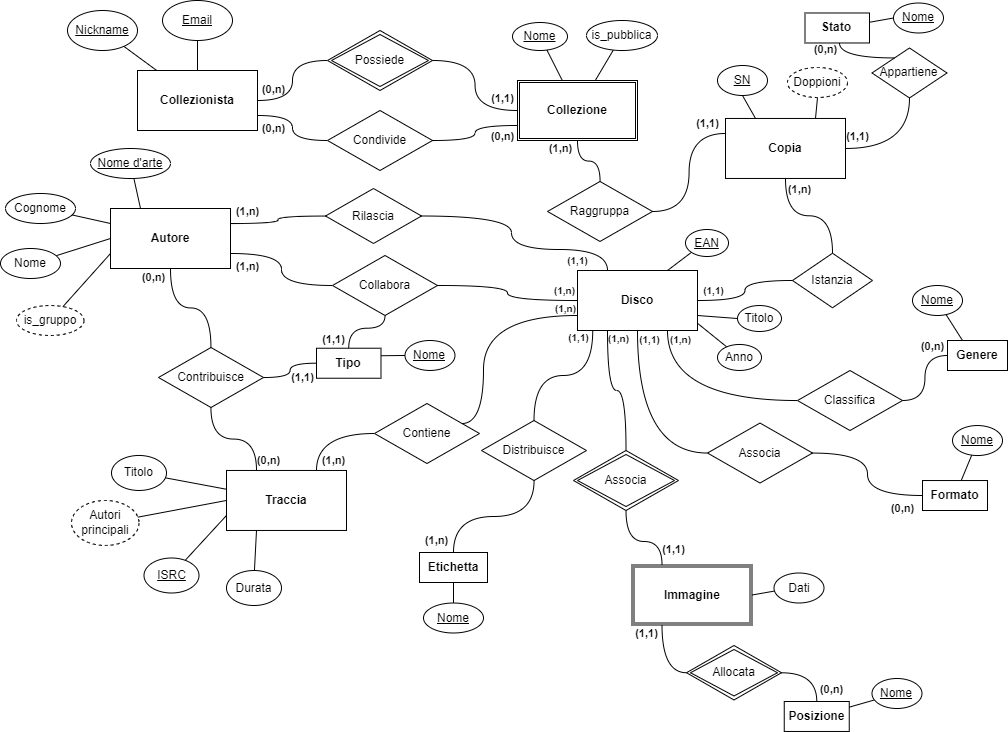
\includegraphics[width=1\linewidth]{ER_ristrutturato_ldb.png}
\end{center}

\subsection{Trasformazioni effettuate}
\begin{enumerate}
    \item Tutti gli attributi enumerativi (genere e formato per l'entità "Disco", stato per l'entità "Copia" e tipo per le relazioni "Contribuisce" e "Rilascia") sono stati trasformati in entità.
    \item In particolare, l'attributo multiplo genere è stato trasformato in una relazione (1,n).
    \item La generalizzazione di "Autore" (singolo e gruppo) è stata rimossa lasciando spazio al flag is\_gruppo ricavabile da nome e cognome (se sono nulli, l'autore è un gruppo).
\end{enumerate}

\pagebreak

\section{Modello relazionale}
\begin{itemize}
    \item \textbf{Collezionista}(\underline{ID}, nickname, email)
          \\[3pt] \textnormal{[nickname UNIQUE, email UNIQUE]}
    \item \textbf{Collezione}(\underline{ID}, nome, isPubblica, id\_Collezionista)
          \\[3pt] \textnormal{[(nome, id\_Collezionista) UNIQUE]}
    \item \textbf{Copia}(\underline{ID}, SN, doppioni, id\_Disco, nome\_Stato, id\_Collezione)
          \\[3pt] \textnormal{[SN UNIQUE]}
    \item \textbf{Disco}(\underline{ID}, EAN, titolo, anno, id\_Etichetta, nome\_Formato, id\_Autore)
          \\[3pt] \textnormal{[EAN UNIQUE, (titolo, anno, id\_Etichetta, nome\_Formato, id\_Autore) UNIQUE]}
    \item \textbf{Autore}(\underline{ID}, nomeDarte, nome, cognome, isGruppo)
          \\[3pt] \textnormal{[nomeDarte UNIQUE, nome NULL, cognome NULL]}
    \item \textbf{Traccia}(\underline{ID}, titolo, ISRC, Durata)
          \\[3pt] \textnormal{[ISRC UNIQUE]}
    \item \textbf{Immagine}(\underline{ID}, dati, id\_Disco, nome\_Posizione)
          \\[3pt] \textnormal{[(id\_Disco, nome\_Posizione) UNIQUE]}
    \item \textbf{Etichetta}(\underline{nome})
    \item \textbf{Stato}(\underline{nome})
    \item \textbf{Genere}(\underline{nome})
    \item \textbf{Formato}(\underline{nome})
    \item \textbf{Posizione}(\underline{nome})
    \item \textbf{Tipo}(\underline{nome})
    \item \textbf{condivide}(\underline{id\_Collezionista}, \underline{id\_Collezione})
    \item \textbf{collabora}(\underline{id\_Autore}, \underline{id\_Disco}, nome\_Tipo)
    \item \textbf{contribuisce}(\underline{id\_Autore}, \underline{id\_Traccia}, nome\_Tipo)
    \item \textbf{contiene}(\underline{id\_Traccia}, \underline{id\_Disco})
    \item \textbf{classifica}(\underline{id\_Disco}, \underline{id\_Genere})
\end{itemize}

\pagebreak
\section{Implementazione della struttura}

\begin{lstlisting}[language=SQL]
    DROP DATABASE IF EXISTS collectors;

    CREATE DATABASE collectors;
    USE collectors;

    DROP USER IF EXISTS 'collectorsUser'@'localhost';
    CREATE USER 'collectorsUser'@'localhost' IDENTIFIED BY 'collectorsPwd';
    GRANT select,insert,update,delete,execute ON collectors.* TO 'collectorsUser'@'localhost';

    CREATE TABLE Collezionista (
        ID INT UNSIGNED AUTO_INCREMENT PRIMARY KEY,
        nickname VARCHAR(50) UNIQUE NOT NULL,
        email VARCHAR(100) UNIQUE NOT NULL
    );

    CREATE TABLE Collezione (
        ID INT UNSIGNED AUTO_INCREMENT PRIMARY KEY,
        nome VARCHAR(50) NOT NULL,
        isPubblica BOOLEAN NOT NULL,
        id_Collezionista INT UNSIGNED NOT NULL,
        CONSTRAINT collezione_distinta UNIQUE (nome, id_Collezionista),
        CONSTRAINT collezione_collezionista FOREIGN KEY (id_Collezionista) REFERENCES Collezionista(ID) ON DELETE CASCADE ON UPDATE CASCADE 
    );

    CREATE TABLE Etichetta (
        nome VARCHAR(50) PRIMARY KEY
    );

    CREATE TABLE Genere (
        nome VARCHAR(50) PRIMARY KEY
    );

    CREATE TABLE Formato (
        nome VARCHAR(50) PRIMARY KEY
    );

    CREATE TABLE Disco (
        ID INT UNSIGNED AUTO_INCREMENT PRIMARY KEY,
        EAN CHAR(13) UNIQUE NOT NULL, 
        --EAN-13 ha una lunghezza fissa di 13 caratteri
        titolo VARCHAR(50) NOT NULL,
        anno SMALLINT UNSIGNED NOT NULL,
        nome_Etichetta VARCHAR(50) NOT NULL,
        nome_Formato VARCHAR(50) NOT NULL,
        id_Autore INT UNSIGNED NOT NULL,
        CONSTRAINT disco_distinto UNIQUE (titolo, anno, nome_Etichetta, nome_Formato, id_Autore), 
        --Non ha senso che esistano dischi uguali con EAN distinti
        CONSTRAINT disco_etichetta FOREIGN KEY (nome_Etichetta) REFERENCES Etichetta(nome) ON DELETE NO ACTION ON UPDATE CASCADE,
        CONSTRAINT disco_formato FOREIGN KEY (nome_Formato) REFERENCES Formato(nome) ON DELETE NO ACTION ON UPDATE CASCADE,
        CONSTRAINT controllo_anno CHECK (anno > 1930 AND anno < 2100) 
        
        --Nel 1931, la casa discografica Rca-Victor distribui il primo Lp della storia: la Quinta sinfonia di Beethoven.
    );

    CREATE TABLE classifica (
        id_Disco INT UNSIGNED,
        nome_Genere VARCHAR(50),
        PRIMARY KEY (id_Disco, nome_Genere),
        CONSTRAINT classifica_disco FOREIGN KEY (id_Disco) REFERENCES Disco(ID) ON DELETE CASCADE ON UPDATE CASCADE,
        CONSTRAINT classifica_genere FOREIGN KEY (nome_Genere) REFERENCES Genere(nome) ON DELETE CASCADE ON UPDATE CASCADE
    );

    CREATE TABLE Stato (
        nome VARCHAR(50) PRIMARY KEY
    );


    -- Facendo riferimento all'assunzione 1, essendo la copia strettamente collegata alla collezione, ritengo corretto eliminare le copie di una collezione quando essa viene eliminata.

    CREATE TABLE Copia (
        ID INT UNSIGNED AUTO_INCREMENT PRIMARY KEY,
        SN CHAR(12) UNIQUE,
        doppioni INT UNSIGNED NOT NULL DEFAULT 1, 
        --Quando si inserisce una copia, il conteggio viene chiaramente inizializzato a uno (ovvero la copia stessa)
        id_Disco INT UNSIGNED NOT NULL,
        nome_Stato VARCHAR(50) NOT NULL,
        id_Collezione INT UNSIGNED NOT NULL,
        CONSTRAINT copia_disco FOREIGN KEY (id_Disco) REFERENCES Disco(ID) ON DELETE NO ACTION ON UPDATE CASCADE,
        CONSTRAINT copia_stato FOREIGN KEY (nome_Stato) REFERENCES Stato(nome) ON DELETE NO ACTION ON UPDATE CASCADE,
        CONSTRAINT copia_collezione FOREIGN KEY (id_Collezione) REFERENCES Collezione(ID) ON DELETE CASCADE ON UPDATE CASCADE 
    );

    CREATE TABLE Autore (
        ID INT UNSIGNED AUTO_INCREMENT PRIMARY KEY,
        nomeDarte VARCHAR(100) UNIQUE NOT NULL,
        nome VARCHAR(100),
        cognome VARCHAR(100),
        isGruppo BOOLEAN NOT NULL
    );


    -- Controllo sul vincolo tra nome, cognome e isGruppo
    DELIMITER $$
    CREATE TRIGGER AggiuntaAutore BEFORE INSERT ON Autore FOR EACH ROW
    BEGIN
        IF NEW.nome IS NOT NULL AND NEW.cognome IS NOT NULL AND NEW.isGruppo = TRUE THEN
            SIGNAL SQLSTATE '45000' SET MESSAGE_TEXT = 'Se nome e cognome non sono nulli, autore deve essere un singolo';
        END IF;
    END$$
    DELIMITER ;


    CREATE TABLE Traccia (
        ID INT UNSIGNED AUTO_INCREMENT PRIMARY KEY,
        titolo VARCHAR(100) NOT NULL,
        ISRC CHAR(12) UNIQUE NOT NULL, 
        -- Codice ISRC composto da 12 cifre alfanumeriche
        Durata TIME NOT NULL
    );

    CREATE TABLE Posizione (
        nome VARCHAR(50) PRIMARY KEY
    );

    CREATE TABLE Immagine (
        ID INT UNSIGNED AUTO_INCREMENT PRIMARY KEY,
        URL VARCHAR(2083),
        id_Disco INT UNSIGNED NOT NULL,
        nome_Posizione VARCHAR(50) NOT NULL,
        CONSTRAINT immagine_distinta UNIQUE (id_Disco, nome_Posizione),
        CONSTRAINT immagine_disco FOREIGN KEY (id_Disco) REFERENCES Disco(ID) ON DELETE CASCADE ON UPDATE CASCADE,
        CONSTRAINT immagine_posizione FOREIGN KEY (nome_Posizione) REFERENCES Posizione(nome) ON DELETE NO ACTION ON UPDATE CASCADE
    );

    CREATE TABLE Tipo (
        nome VARCHAR(50) PRIMARY KEY
    );

    CREATE TABLE condivide (
        id_Collezionista INT UNSIGNED,
        id_Collezione INT UNSIGNED,
        PRIMARY KEY (id_Collezionista, id_Collezione),
        CONSTRAINT condivide_collezionista FOREIGN KEY (id_Collezionista) REFERENCES Collezionista(ID) ON DELETE CASCADE ON UPDATE CASCADE,
        CONSTRAINT condivide_collezione FOREIGN KEY (id_Collezione) REFERENCES Collezione(ID) ON DELETE CASCADE ON UPDATE CASCADE
    );

    CREATE TABLE collabora (
        id_Autore INT UNSIGNED,
        id_Disco INT UNSIGNED,
        nome_Tipo VARCHAR(50) NOT NULL,
        PRIMARY KEY (id_Autore, id_Disco),
        CONSTRAINT collabora_autore FOREIGN KEY (id_Autore) REFERENCES Autore(ID) ON DELETE NO ACTION ON UPDATE CASCADE,
        CONSTRAINT collabora_disco FOREIGN KEY (id_Disco) REFERENCES Disco(ID) ON DELETE CASCADE ON UPDATE CASCADE,
        CONSTRAINT collabora_tipo FOREIGN KEY (nome_Tipo) REFERENCES Tipo(nome) ON DELETE NO ACTION ON UPDATE CASCADE
    );
        
    CREATE TABLE contribuisce (
        id_Autore INT UNSIGNED,
        id_Traccia INT UNSIGNED,
        nome_Tipo VARCHAR(50) NOT NULL,
        PRIMARY KEY (id_Autore, id_Traccia),
        CONSTRAINT contribuisce_autore FOREIGN KEY (id_Autore) REFERENCES Autore(ID) ON DELETE CASCADE ON UPDATE CASCADE,
        CONSTRAINT contribuisce_traccia FOREIGN KEY (id_Traccia) REFERENCES Traccia(ID) ON DELETE CASCADE ON UPDATE CASCADE,
        CONSTRAINT contribuisce_tipo FOREIGN KEY (nome_Tipo) REFERENCES Tipo(nome) ON DELETE NO ACTION ON UPDATE CASCADE
        );
        
        CREATE TABLE contiene (
        id_Traccia INT UNSIGNED,
        id_Disco INT UNSIGNED,
        PRIMARY KEY (id_Traccia, id_Disco),
        CONSTRAINT contiene_traccia FOREIGN KEY (id_Traccia) REFERENCES Traccia(ID) ON DELETE CASCADE ON UPDATE CASCADE,
        CONSTRAINT contiene_disco FOREIGN KEY (id_Disco) REFERENCES Disco(ID) ON DELETE CASCADE ON UPDATE CASCADE
        );
        
    \end{lstlisting}
    \pagebreak

    \section{Operazioni richieste}
    In questa sezione troviamo le operazioni richieste al database. Ogni operazione è inclusa in una procedura e nella prima parte sono presenti delle procedure ausiliarie che ho utilizzato durante lo sviluppo.
    All'inizio del documento sono presenti le seguenti righe di codice:

    \begin{lstlisting}[language=SQL]
    USE collectors;
    DELIMITER $$
\end{lstlisting}

\subsection{Procedure ausiliarie}


\subsubsection{Stampa ogni coppia disco-traccia con i relativi attributi}
\begin{lstlisting}[language=SQL]
    DROP PROCEDURE IF EXISTS DischiTracce$$
    
    CREATE PROCEDURE DischiTracce() 
    BEGIN
    SELECT D.titolo as "Titolo Disco", D.EAN, T.titolo as "Titolo Traccia", T.ISRC, T.durata, A.nomeDarte as "Autore principale" FROM Disco D, Traccia T, Contiene C, Autore A WHERE D.id = C.id_disco AND T.id = C.id_traccia AND A.id = D.id_autore ORDER BY D.titolo;
    END$$
\end{lstlisting}

\subsubsection{Stampa ogni coppia collezione-collezionista delle condivisioni}
\begin{lstlisting}[language=SQL]
    DROP PROCEDURE IF EXISTS Condivisioni$$
    
    CREATE PROCEDURE Condivisioni()
    BEGIN
        SELECT C.nickname as "Owner", CL.nome as "Collezione", C2.nickname as "Guest" FROM Collezionista C, Collezione CL, Collezionista C2, Condivide CO WHERE CL.isPubblica = false AND CL.id_collezionista = C.id AND CL.id = CO.id_collezione AND C2.id = CO.id_collezionista;
    END$$
\end{lstlisting}

\subsubsection{Stampa ogni coppia collezione-copia}
\begin{lstlisting}[language=SQL]
    DROP PROCEDURE IF EXISTS CollezioniCopie$$

    CREATE PROCEDURE CollezioniCopie()
    BEGIN
        SELECT CL.nickname, C.nome, CO.SN, CO.nome_Stato AS "Stato", CO.doppioni, C.isPubblica AS Pubblica, D.titolo, D.EAN, A.nomeDarte AS "Autore principale" FROM Autore A, Collezionista CL, Collezione C, Copia CO, Disco D WHERE C.id = CO.id_collezione AND CO.id_disco = D.id AND C.id_collezionista = CL.id AND A.id = D.id_autore ORDER BY C.nome;
    END$$    
\end{lstlisting}

\subsubsection{Stampa ogni coppia disco-copia}
\begin{lstlisting}[language=SQL]
    DROP PROCEDURE IF EXISTS DischiCopie$$

    CREATE PROCEDURE DischiCopie()
    BEGIN
        SELECT D.titolo, D.EAN, C.SN, C.nome_Stato, A.nomeDarte AS "Autore principale" FROM Disco D, Copia C, Autore A WHERE C.id_disco = D.id AND A.id = D.id_autore;
    END$$
\end{lstlisting}

\subsubsection{Stampa ogni coppia disco-autore secondario}
\begin{lstlisting}[language=SQL]
    DROP PROCEDURE IF EXISTS DischiAutoriSec$$

    CREATE PROCEDURE DischiAutoriSec()
    BEGIN
        SELECT D.titolo, D.EAN, A.nomeDarte AS "Autore Secondario", C.nome_tipo AS "Tipo" FROM Disco D, Autore A, Collabora C WHERE D.id = C.id_disco AND C.id_autore = A.id;
    END$$
\end{lstlisting}

\subsubsection{Stampa ogni coppia traccia-autore secondario}
\begin{lstlisting}[language=SQL]
    DROP PROCEDURE IF EXISTS TracceAutoriSec$$

    CREATE PROCEDURE TracceAutoriSec()
    BEGIN
        SELECT T.titolo, t.ISRC, A.nomeDarte AS "Autore Secondario", C.nome_tipo AS "Tipo" FROM Traccia T, Autore A, Contribuisce C WHERE T.id = C.id_traccia AND C.id_autore = A.id;
    END$$
\end{lstlisting}

\subsubsection{Dato nome della collezione e nickname del collezionista, restituisce l'id della collezione}
\begin{lstlisting}[language=SQL]
    DROP FUNCTION IF EXISTS GetCollezione$$

    CREATE FUNCTION GetCollezione (
        p_nome_collezione VARCHAR(50),
        p_nickname_collezionista VARCHAR(50)
    ) RETURNS INT UNSIGNED DETERMINISTIC
    BEGIN
        RETURN (SELECT id FROM Collezione WHERE nome = p_nome_collezione AND id_collezionista = (SELECT id FROM Collezionista WHERE nickname = p_nickname_collezionista));
    END$$
    \end{lstlisting}

\subsection*{1. Inserimento di una nuova collezione}
\begin{lstlisting}[language=SQL]
    DROP PROCEDURE IF EXISTS InserisciCollezione$$

    CREATE PROCEDURE InserisciCollezione(
        IN p_nome VARCHAR(50),
        IN p_isPubblica BOOLEAN,
        IN p_nickname_collezionista VARCHAR(50)
    )
    BEGIN
        DECLARE p_id_collezionista INT UNSIGNED;
        SET p_id_collezionista = (SELECT id FROM Collezionista WHERE nickname = p_nickname_collezionista);
        
        IF p_id_collezionista IS NULL THEN
            SIGNAL SQLSTATE '45000' SET MESSAGE_TEXT = 'Non esiste un collezionista con questo nickname';
        ELSE
        -- Inserimento della nuova riga nella tabella Collezione
            INSERT INTO Collezione (nome, isPubblica, id_Collezionista)
            VALUES (p_nome, p_isPubblica, p_id_Collezionista);
        END IF;
    END$$
    \end{lstlisting}

\subsection*{2. Aggiunta di dischi a una collezione e di tracce a un disco}

\subsubsection*{2a. Inserimento di un disco non presente nel sistema}
\begin{lstlisting}[language=SQL]
    CREATE PROCEDURE InserisciDisco(
        IN p_EAN CHAR(13),
        IN p_titolo VARCHAR(50),
        IN p_anno SMALLINT,
        IN p_nome_Etichetta VARCHAR(50),
        IN p_nome_Formato VARCHAR(50),
        IN p_nomeDarte_autore_principale VARCHAR(50),
        IN p_nome_genere_principale VARCHAR(50)
    )
    BEGIN
        DECLARE p_id_autore INT UNSIGNED;
        DECLARE p_id_nuovo_disco INT UNSIGNED;
        SET p_id_autore = (SELECT id FROM Autore WHERE nomeDarte = p_nomeDarte_autore_principale);
        
        IF p_id_autore IS NULL THEN
            SIGNAL SQLSTATE '45000' SET MESSAGE_TEXT = 'Non esiste un autore con questo nome d arte';
        ELSEIF (SELECT * FROM Genere WHERE nome = p_nome_genere_principale) IS NULL THEN
            SIGNAL SQLSTATE '45000' SET MESSAGE_TEXT = 'Il genere indicato non esiste';
        ELSE
            IF (SELECT * FROM Etichetta WHERE nome = p_nome_Etichetta) IS NULL THEN
                INSERT INTO Etichetta VALUE (p_nome_Etichetta);
            END IF;
            INSERT INTO Disco(EAN,titolo,anno,nome_Etichetta,nome_Formato,id_Autore) VALUE (p_EAN,p_titolo,p_anno,p_nome_Etichetta,p_nome_Formato,p_id_autore);
            SET p_id_nuovo_disco = last_insert_id();
            INSERT INTO Classifica VALUE (p_id_nuovo_disco, p_nome_genere_principale);
        END IF;
    END$$
\end{lstlisting}
        
\subsubsection*{2b. Aggiunta di un genere secondario al disco}
\begin{lstlisting}[language=SQL]
    DROP PROCEDURE IF EXISTS AggiungiGenereAlDisco$$

    CREATE PROCEDURE AggiungiGenereAlDisco(
        IN p_nome_genere VARCHAR(50),
        IN p_EAN_disco CHAR(13)
    )
    BEGIN
        IF (SELECT * FROM Genere WHERE nome = p_nome_genere) IS NULL THEN	
            SIGNAL SQLSTATE '45000' SET MESSAGE_TEXT = 'Non esiste un genere con questo nome';
        ELSEIF (SELECT id FROM Disco WHERE EAN = p_EAN_disco) IS NULL THEN
            SIGNAL SQLSTATE '45000' SET MESSAGE_TEXT = 'Non esiste un disco con questo EAN';
        ELSEIF EXISTS (SELECT * FROM Classifica WHERE id_disco = (SELECT id FROM Disco WHERE EAN = p_EAN_disco) AND nome_genere = p_nome_genere) THEN
            SIGNAL SQLSTATE '45000' SET MESSAGE_TEXT = 'Genere gia associato al disco';
        ELSE
            INSERT INTO Classifica VALUE ((SELECT id FROM Disco WHERE EAN = p_EAN_disco), p_nome_genere);
        END IF;
    END$$
\end{lstlisting}
        
\subsubsection*{2c. Aggiunta autore secondario al disco}
\begin{lstlisting}[language=SQL]
    DROP PROCEDURE IF EXISTS AggiungiAutoreAlDisco$$

    CREATE PROCEDURE AggiungiAutoreAlDisco(
        IN p_nomeDarte_autore VARCHAR(50),
        IN p_EAN_disco CHAR(13),
        IN p_nome_tipo VARCHAR(50)
    )
    BEGIN
        DECLARE p_id_autore INT UNSIGNED;
        DECLARE p_id_disco INT UNSIGNED;
        SET p_id_autore = (SELECT id FROM Autore WHERE nomeDarte = p_nomeDarte_autore);
        SET p_id_disco = (SELECT id FROM Disco WHERE EAN = p_EAN_disco);
        IF p_id_autore IS NULL THEN	
            SIGNAL SQLSTATE '45000' SET MESSAGE_TEXT = 'L autore indicato non esiste';
        ELSEIF p_id_disco IS NULL THEN
            SIGNAL SQLSTATE '45000' SET MESSAGE_TEXT = 'Non esiste un disco con questo EAN';
        ELSEIF (SELECT * FROM Tipo WHERE nome = p_nome_tipo) IS NULL THEN
            SIGNAL SQLSTATE '45000' SET MESSAGE_TEXT = 'Non esiste un tipo con questo nome';
        ELSEIF EXISTS ((SELECT * FROM collabora WHERE id_disco = p_id_disco AND id_autore = p_id_autore AND nome_Tipo = p_nome_tipo)) THEN
            SIGNAL SQLSTATE '45000' SET MESSAGE_TEXT = 'Autore gia associato al disco in quel ruolo';
        ELSEIF EXISTS (SELECT id FROM Disco WHERE id_autore = p_id_autore and id = p_id_disco) THEN 
            SIGNAL SQLSTATE '45000' SET MESSAGE_TEXT = 'Autore gia associato al disco in quel ruolo';
        ELSE
            INSERT INTO collabora VALUE (p_id_autore, p_id_disco, p_nome_tipo);
        END IF;
    END$$
\end{lstlisting}
            
\subsubsection*{2d. Aggiunta di nuova copia ed assegnamento ad una collezione}
\begin{lstlisting}[language=SQL]
    DROP PROCEDURE IF EXISTS InserisciCopia$$

    CREATE PROCEDURE InserisciCopia(
        IN p_SN CHAR(12),
        IN p_EAN_Disco CHAR(13),
        IN p_nome_Stato VARCHAR(50),
        IN p_nome_Collezione VARCHAR(50),
        IN p_nickname_Collezionista VARCHAR(50)
    )
    BEGIN
        DECLARE num_doppioni INT;
        DECLARE p_id_Disco INT UNSIGNED;
        DECLARE p_id_collezione INT UNSIGNED;
        SET p_id_Disco = (SELECT D.id FROM Disco D WHERE D.EAN = p_EAN_Disco);
        SET p_id_collezione = GetCollezione(p_nome_collezione, p_nickname_Collezionista);
        IF EXISTS (SELECT id FROM Copia WHERE SN = p_SN) THEN
            SIGNAL SQLSTATE '45000' SET MESSAGE_TEXT = 'Esiste gia una copia con questo SN';
        ELSEIF p_id_Disco IS NULL THEN 
            SIGNAL SQLSTATE '45000' SET MESSAGE_TEXT = 'Non esiste un disco con questo EAN';
        ELSEIF p_id_collezione IS NULL THEN
            SIGNAL SQLSTATE '45000' SET MESSAGE_TEXT = 'Non esiste una collezione con questo nome associata a questo nickname';
        ELSE    
            -- Inserimento della nuova riga nella tabella Copia
            INSERT INTO Copia (SN, id_Disco, nome_Stato, id_Collezione) 
            VALUES (p_SN, p_id_Disco, p_nome_Stato, p_id_Collezione);
        
            -- Calcolo del numero di doppioni per l'id_disco appena inserito
            SET num_doppioni = (SELECT COUNT(*) FROM Copia WHERE id_Disco = p_id_Disco);
            
            -- Aggiornamento della colonna doppioni per tutte le copie con lo stesso id_disco
            UPDATE Copia C
            SET C.doppioni = num_doppioni
            WHERE C.id_Disco = p_id_Disco;
        END IF;
    END$$
\end{lstlisting}
                
\subsubsection*{2e. Spostamento copia gia esistente da una collezione ad un altra dello stesso utente}
\begin{lstlisting}[language=SQL]
    DROP PROCEDURE IF EXISTS CopiaInCollezione$$

    CREATE PROCEDURE CopiaInCollezione(
        IN p_nome_collezione VARCHAR(50),
        IN p_SN_copia CHAR(12)
    )
    BEGIN
        DECLARE p_id_collezionista INT UNSIGNED;
        SET p_id_collezionista = (SELECT CZ.id_Collezionista FROM Copia C, Collezione CZ WHERE C.SN = p_SN_copia AND CZ.id = C.id_Collezione);
        
        -- Un collezionista non puo spostare una sua copia nella collezione di un altro utente
        IF EXISTS(SELECT CZ.nome FROM Copia C, Collezione CZ WHERE C.SN = p_SN_copia AND C.id_collezione = CZ.id AND CZ.nome = p_nome_collezione AND CZ.id_collezionista = p_id_collezionista) THEN
            SIGNAL SQLSTATE '45000' SET MESSAGE_TEXT = 'Copia gia nella collezione';
        ELSEIF EXISTS(SELECT CZ.nome FROM Collezione CZ WHERE CZ.nome = p_nome_collezione AND CZ.id_collezionista = p_id_collezionista) THEN
            UPDATE Copia C
            SET C.id_Collezione = (SELECT C.id FROM Collezione C, Collezionista CL WHERE C.nome = p_nome_collezione AND CL.id = p_id_collezionista)
            WHERE C.SN = p_SN_copia;
        ELSE
            SIGNAL SQLSTATE '45000' SET MESSAGE_TEXT = 'La collezione indicata non esiste';
        END IF;
    END$$
\end{lstlisting}
    
\subsubsection*{2f. inserimento di una nuova traccia ed assegnamento a un disco esistente}
\begin{lstlisting}[language=SQL]
    DROP PROCEDURE IF EXISTS NuovaTracciaInDisco$$

    CREATE PROCEDURE NuovaTracciaInDisco(
        p_titolo VARCHAR(100),
        p_ISRC CHAR(12),
        p_durata TIME,
        p_EAN CHAR(13)
    )
    BEGIN
        DECLARE p_id_disco INT UNSIGNED;
        DECLARE p_id_nuova_traccia INT UNSIGNED;
        SET p_id_disco = (SELECT D.id FROM Disco D WHERE D.EAN = p_EAN);
        
        IF p_id_disco IS NULL THEN
            SIGNAL SQLSTATE '45000' SET MESSAGE_TEXT = 'Il disco indicato non esiste'; 
        ELSE
            INSERT INTO Traccia(titolo, ISRC, durata) VALUES (p_titolo, p_ISRC, p_durata);
            SET p_id_nuova_traccia = last_insert_id();
            INSERT INTO Contiene VALUES (p_id_nuova_traccia,p_id_disco);
        END IF;
    END$$
\end{lstlisting}
        
\subsubsection*{2g. Inserimento traccia esistente in un disco}
\begin{lstlisting}[language=SQL]
    DROP PROCEDURE IF EXISTS TracciaInDisco$$

    CREATE PROCEDURE TracciaInDisco(
        IN p_ISRC_traccia CHAR(12),
        IN p_EAN_disco CHAR(13)
    )
    BEGIN
        DECLARE p_id_traccia INT UNSIGNED;
        DECLARE p_id_disco INT UNSIGNED;
        SET p_id_traccia = (SELECT T.id FROM Traccia T WHERE T.ISRC = p_ISRC_traccia);
        SET p_id_disco = (SELECT D.id FROM Disco D WHERE D.EAN = p_EAN_disco);
        
        IF p_id_disco IS NULL THEN
            SIGNAL SQLSTATE '45000' SET MESSAGE_TEXT = 'Il disco indicato non esiste';
        ELSEIF p_id_traccia IS NULL THEN
            SIGNAL SQLSTATE '45000' SET MESSAGE_TEXT = 'La traccia indicata non esiste';
        ELSEIF EXISTS (SELECT C.* FROM Contiene C WHERE C.id_traccia = p_id_traccia AND C.id_disco = p_id_disco) THEN
            SIGNAL SQLSTATE '45000' SET MESSAGE_TEXT = 'Traccia gia nel disco';
        ELSE
            INSERT INTO Contiene (id_traccia, id_disco) VALUES (p_id_traccia, p_id_disco);
        END IF;
    END$$
\end{lstlisting}
    
\subsection*{3. Modifica dello stato di pubblicazione e aggiunta nuove condivisioni}
\subsubsection*{3a. Modifica dello stato di condivisione}
\begin{lstlisting}[language=SQL]
    DROP PROCEDURE IF EXISTS switchCondivisione$$

    CREATE PROCEDURE switchCondivisione(
        IN p_nome_Collezione VARCHAR(50),
        IN p_nickname_Collezionista VARCHAR(50)
    )
    BEGIN
        DECLARE p_stato_attuale BOOLEAN;
        DECLARE p_id_collezione INT UNSIGNED;
        
        SET p_id_collezione = GetCollezione(p_nome_Collezione, p_nickname_Collezionista);
        SET p_stato_attuale = (SELECT isPubblica FROM Collezione WHERE id = p_id_collezione);
        
        UPDATE Collezione SET isPubblica = NOT p_stato_attuale WHERE id = p_id_collezione;
        
        IF p_id_collezione IS NULL THEN 
            SIGNAL SQLSTATE '45000' SET MESSAGE_TEXT = 'La collezione non esiste';
        ELSEIF (p_stato_attuale = TRUE) THEN
            DELETE FROM condivide WHERE id_collezione = p_id_collezione;
            # Se sto switchando da Privata a Pubblica, rimuovo i collezionisti con cui era condivisa
        END IF;
    END$$
\end{lstlisting}

\subsubsection*{3a. Aggiunta di una nuova condivisione (se privata)}
\begin{lstlisting}[language=SQL]
    DROP PROCEDURE IF EXISTS AggiungiCondivisione$$
    
    CREATE PROCEDURE AggiungiCondivisione(
        IN p_nickname_owner VARCHAR(50),
        IN p_nickname_guest VARCHAR(50),
        IN p_nome_collezione VARCHAR(50)
        )
    BEGIN
        DECLARE p_id_collezione INT UNSIGNED;
        DECLARE p_id_owner INT UNSIGNED;
        DECLARE p_id_guest INT UNSIGNED;
        
        SET p_id_owner = (SELECT id FROM Collezionista WHERE nickname = p_nickname_owner);
        
        IF p_id_owner IS NULL THEN
        SIGNAL SQLSTATE '45000' SET MESSAGE_TEXT = 'Non esiste un utente con il nickname indicato per l owner';
        ELSE
            SET p_id_collezione = (SELECT id FROM Collezione WHERE nome = p_nome_collezione AND id_collezionista = p_id_owner);
            
            IF p_id_collezione IS NULL THEN
                SIGNAL SQLSTATE '45000' SET MESSAGE_TEXT = 'La collezione non esiste';
                ELSE
                SET p_id_guest = (SELECT id FROM Collezionista WHERE nickname = p_nickname_guest);
                
                IF p_id_guest IS NULL THEN
                SIGNAL SQLSTATE '45000' SET MESSAGE_TEXT = 'Non esiste un utente con il nickname indicato per il guest';
                ELSE
                IF (SELECT isPubblica FROM Collezione WHERE id = p_id_collezione) = TRUE THEN
                SIGNAL SQLSTATE '45000' SET MESSAGE_TEXT = 'collezione pubblica, renderla privata e riprovare';
                ELSE
                IF EXISTS (SELECT * FROM Condivide WHERE id_collezionista = p_id_guest AND id_collezione = p_id_collezione) THEN
                SIGNAL SQLSTATE '45000' SET MESSAGE_TEXT = 'Collezione gia condivisa con questo utente';
                ELSE
                INSERT INTO Condivide VALUES (p_id_guest, p_id_collezione);
                END IF;
                    END IF;
                    END IF;
            END IF;
            END IF;
    END$$
\end{lstlisting}

\subsection*{4. Rimozione di un disco da una collezione}
\begin{lstlisting}[language=SQL]
    DROP PROCEDURE IF EXISTS RimuoviCopiaDaCollezione$$

    -- Come detto nell'assunzione 1, ritengo poco utile mantenere nel sistema copie senza una collezione. Di conseguenza, rimuovere una copia da una collezione significa rimuoverla dal sistema.
    
    CREATE PROCEDURE RimuoviCopiaDaCollezione(
        p_SN_copia CHAR(12),
        p_nome_collezione VARCHAR(50)
    )
    BEGIN
        DECLARE p_id_copia INT UNSIGNED;
        DECLARE p_id_collezione INT UNSIGNED;
        SET p_id_copia = (SELECT id FROM Copia WHERE SN = p_SN_copia); 
        IF p_id_copia IS NULL THEN 
            SIGNAL SQLSTATE '45000' SET MESSAGE_TEXT = 'Non esiste una copia con questo SN';
        ELSE 
            SET p_id_collezione = (SELECT C.id FROM Collezione C, Copia CP WHERE CP.id = p_id_copia AND C.id = CP.id_collezione AND C.nome = p_nome_collezione);
            IF p_id_collezione IS NULL THEN
                SIGNAL SQLSTATE '45000' SET MESSAGE_TEXT = 'La copia non fa parte della collezione indicata';
            ELSE 
                DELETE FROM Copia WHERE id = p_id_copia;
            END IF;
        END IF;
    END$$
\end{lstlisting}

\subsection*{5. Rimozione di una collezione}
\begin{lstlisting}[language=SQL]
    DROP PROCEDURE IF EXISTS RimuoviCollezione$$

    CREATE PROCEDURE RimuoviCollezione(
        p_nickname_collezionista VARCHAR(50),
        p_nome_collezione VARCHAR(50)
    )
    BEGIN
        DECLARE p_id_collezione INT UNSIGNED;
        SET p_id_collezione = GetCollezione(p_nome_collezione, p_nickname_collezionista);
        
        IF p_id_collezione IS NULL THEN
            SIGNAL SQLSTATE '45000' SET MESSAGE_TEXT = 'La collezione indicata non esiste';
        ELSE
            DELETE FROM Collezione WHERE id = p_id_collezione;
        END IF;
    END$$
    
\end{lstlisting}

\subsection*{6. Lista di tutti i dischi in una collezione}
\begin{lstlisting}[language=SQL]
    DROP PROCEDURE IF EXISTS DischiInCollezione$$
    
    CREATE PROCEDURE DischiInCollezione(
        p_nickname_collezionista VARCHAR(50),
        p_nome_collezione VARCHAR(50)
    )
    BEGIN
        DECLARE p_id_collezione INT UNSIGNED;
        SET p_id_collezione = GetCollezione(p_nome_collezione, p_nickname_collezionista);
        
        IF p_id_collezione IS NULL THEN
            SIGNAL SQLSTATE '45000' SET MESSAGE_TEXT = 'La collezione indicata non esiste';
        ELSE
            SELECT DISTINCT D.* FROM Disco D, Copia C WHERE D.id = C.id_disco AND C.id_collezione = p_id_collezione;
        END IF;
    END$$
\end{lstlisting}

\subsection*{7. Track list di un disco}
\begin{lstlisting}[language=SQL]
    
    DROP PROCEDURE IF EXISTS TrackList$$
    
    CREATE PROCEDURE TrackList(
        p_EAN CHAR(13)
    )
    BEGIN
        DECLARE p_id_disco INT UNSIGNED;
        SET p_id_disco = (SELECT id FROM Disco WHERE EAN = p_EAN);
        
        IF p_id_disco IS NULL THEN
            SIGNAL SQLSTATE '45000' SET MESSAGE_TEXT = 'Il disco indicato non esiste';
        ELSE
            SELECT DISTINCT T.* FROM Traccia T, Contiene C WHERE C.id_traccia = T.id AND C.id_disco = p_id_disco;
        END IF;
    END$$
\end{lstlisting}

\subsection*{8. Ricerca dischi in base a diversi criteri}
\begin{lstlisting}[language=SQL]
    DROP PROCEDURE IF EXISTS RicercaDischi$$
    
    -- Per non includere l autore nella ricerca, inserisco null come argomento dell'autore. Stesso discorso per il titolo.
    CREATE PROCEDURE RicercaDischi(
        IN p_nome_autore VARCHAR(50),
        IN p_titolo VARCHAR(50),
        IN p_nome_collezionista VARCHAR(50),
        IN p_includi_private BOOLEAN,
        IN p_includi_condivise BOOLEAN,
        IN p_includi_pubbliche BOOLEAN
    )
    BEGIN
        DECLARE p_id_collezionista INT UNSIGNED;
        DECLARE p_id_autore INT UNSIGNED;
        SET p_id_collezionista = (SELECT id FROM Collezionista WHERE nickname = p_nome_collezionista);
    
        SET p_id_autore = (SELECT id FROM Autore WHERE nomeDarte = p_nome_autore);
        IF p_id_autore IS NULL AND p_nome_autore IS NOT NULL THEN 
            SIGNAL SQLSTATE '45000' SET MESSAGE_TEXT = 'L autore indicato non esiste';
        ELSE
            -- Ricerca in base ai criteri specificati 
            SELECT DISTINCT D.* FROM Disco D, collabora C WHERE 
            ((p_titolo IS NOT NULL AND p_id_autore IS NULL AND D.titolo LIKE CONCAT('%', p_titolo, '%')) 
            OR 
            (p_id_autore IS NOT NULL AND p_titolo IS NULL AND C.id_autore = p_id_autore AND D.id = C.id_disco) 
            OR 
            (p_titolo IS NOT NULL AND p_id_autore IS NOT NULL AND D.titolo LIKE CONCAT('%', p_titolo, '%') AND C.id_autore = p_id_autore AND D.id = C.id_disco))
            AND 
            ((p_includi_private = 1 AND EXISTS (SELECT * FROM Copia C WHERE C.id_disco = D.id AND C.id_collezione IN (SELECT id FROM Collezione WHERE id_collezionista = p_id_collezionista)))
            OR 
            (p_includi_condivise = 1 AND EXISTS (SELECT * FROM Copia C, Condivide CC WHERE C.id_disco = D.id AND C.id_collezione = CC.id_collezione AND CC.id_collezionista = p_id_collezionista))
            OR 
            (p_includi_pubbliche = 1 AND EXISTS (SELECT * FROM Copia C, Collezione CZ WHERE C.id_disco = D.id AND C.id_collezione = CZ.id AND CZ.isPubblica = 1 AND CZ.id_collezionista != p_id_collezionista))); -- escludo le collezioni pubbliche che appartengono al collezionista che fa la query
        END IF;
    END$$
\end{lstlisting}

\subsection*{9. Verifica visibilità collezione}
\begin{lstlisting}[language=SQL]
    DROP PROCEDURE IF EXISTS CheckVisibilita$$
    
    CREATE PROCEDURE CheckVisibilita(
        IN p_nome_collezione VARCHAR(50),
        IN p_nickname_owner VARCHAR(50),
        IN p_nickname_guest VARCHAR(50)
    )
    BEGIN
        DECLARE p_id_collezione INT UNSIGNED;
        SET p_id_collezione = GetCollezione(p_nome_collezione, p_nickname_owner);
        
        IF (SELECT id FROM Collezionista WHERE nickname = p_nickname_guest) IS NULL THEN
            SIGNAL SQLSTATE '45000' SET MESSAGE_TEXT = 'Il collezionista indicato non esiste';
        ELSEIF p_id_collezione IS NULL THEN
            SIGNAL SQLSTATE '45000' SET MESSAGE_TEXT = 'La collezione indicata non esiste';
        ELSE
            IF (SELECT ((p_nickname_owner = p_nickname_guest) OR (SELECT isPubblica FROM Collezione WHERE id = p_id_collezione) = TRUE OR EXISTS (SELECT * FROM Condivide WHERE id_collezione = p_id_collezione AND id_collezionista = (SELECT id FROM Collezionista WHERE nickname = p_nickname_guest)))) = true THEN
                    SELECT "Visibile" AS Risultato;
                ELSE
                    SELECT "Non visibile" AS Risultato;
                END IF;    
        END IF;
    END$$
\end{lstlisting}

\subsection*{10. Numero di brani di un autore nelle collezioni pubbliche}
\begin{lstlisting}[language=SQL]
    DROP PROCEDURE IF EXISTS ContaBraniByAutore$$

    CREATE PROCEDURE ContaBraniByAutore(
        IN p_nomeDarte VARCHAR(50)
    )
    BEGIN
        DECLARE p_id_autore INT UNSIGNED;
        SET p_id_autore = (SELECT id FROM Autore WHERE nomeDarte = p_nomeDarte);
        
        IF p_id_autore IS NULL THEN
            SIGNAL SQLSTATE '45000' SET MESSAGE_TEXT = 'L autore indicato non esiste';
        ELSE
            SELECT count(DISTINCT T.id) AS "Numero tracce" FROM Traccia T, Disco D, Contiene C, Collezione CZ, Copia CO, Contribuisce CB, Collabora CL WHERE 
                ((T.id = CB.id_traccia AND CB.id_autore = p_id_autore) OR (D.id = CL.id_disco AND CL.id_autore = p_id_autore AND T.id = C.id_traccia AND C.id_disco = D.id) OR (D.id_autore = p_id_autore AND T.id = C.id_traccia AND C.id_disco = D.id)) AND 
                T.id = C.id_traccia AND C.id_disco = D.id AND CO.id_disco = D.id AND CO.id_collezione = CZ.id AND CZ.isPubblica = true;
        END IF;
    END$$
\end{lstlisting}

\subsection*{11. Tempo di musica di un autore nelle collezioni pubbliche}
\begin{lstlisting}[language=SQL]
    DROP PROCEDURE IF EXISTS TempoBraniByAutore$$
    
    CREATE PROCEDURE TempoBraniByAutore(
        IN p_nomeDarte VARCHAR(50)
    )
    BEGIN
        DECLARE p_id_autore INT UNSIGNED;
        SET p_id_autore = (SELECT id FROM Autore WHERE nomeDarte = p_nomeDarte);
        
        IF p_id_autore IS NULL THEN
            SIGNAL SQLSTATE '45000' SET MESSAGE_TEXT = 'L autore indicato non esiste';
        ELSE
            SELECT SEC_TO_TIME(SUM(TIME_TO_SEC(durata))) AS "Tempo di musica"
                FROM (SELECT DISTINCT T.id, T.durata AS durata FROM Traccia T, Disco D, Contiene C, Collezione CZ, Copia CO, Contribuisce CB, Collabora CL WHERE 
                ((T.id = CB.id_traccia AND CB.id_autore = p_id_autore) OR (D.id = CL.id_disco AND CL.id_autore = p_id_autore AND T.id = C.id_traccia AND C.id_disco = D.id) OR (D.id_autore = p_id_autore AND T.id = C.id_traccia AND C.id_disco = D.id)) AND 
                T.id = C.id_traccia AND C.id_disco = D.id AND CO.id_disco = D.id AND CO.id_collezione = CZ.id AND CZ.isPubblica = true) as SubQuery;
        END IF;
    END$$
\end{lstlisting}

\subsection*{12a. Numero di collezioni di ciascun collezionista}
\begin{lstlisting}[language=SQL]
    DROP PROCEDURE IF EXISTS ContaCollezioni$$ 

    CREATE PROCEDURE ContaCollezioni()
    BEGIN
        SELECT C.nickname, count(DISTINCT CO.id) as "Numero" FROM Collezionista C, Collezione CO WHERE CO.id_collezionista = C.id GROUP BY C.id;
    END$$
\end{lstlisting}

\subsection*{12b. Numero di dischi per genere}
\begin{lstlisting}[language=SQL]
    DROP PROCEDURE IF EXISTS ContaDischiPerGenere$$

    CREATE PROCEDURE ContaDischiPerGenere()
    BEGIN
        SELECT G.nome, count(DISTINCT D.id) as "Numero" FROM Genere G, Classifica C, Disco D WHERE C.id_disco = D.id AND C.nome_genere = G.nome GROUP BY G.nome;
    END$$
\end{lstlisting}

\subsection*{13. Ricerca coerente con i dati in input}
\begin{lstlisting}[language=SQL]
    DROP PROCEDURE IF EXISTS RicercaCoerente$$

    CREATE PROCEDURE RicercaCoerente(
        IN p_EAN CHAR(13),
        IN p_titolo VARCHAR(50),
        IN p_nomeDarte VARCHAR(50)
    )
    -- Utilizzo due volte soundex per rendere il range di compatibilita piu ampio, l'ordine delle query e definito dall ordine di importanza dei criteri usati
    BEGIN
        IF p_titolo = "" THEN 
            SET p_titolo = null; -- altrimenti cercando con il titolo vuoto mi verrebbero restituiti tutti i dischi del sistema
        END IF;
        
        IF p_nomeDarte = "" THEN
            SET p_nomeDarte = null; -- altrimenti cercando con il nome d'arte vuoto mi verrebbero restituiti tutti i dischi del sistema
        END IF;
        
        -- MATCH con i dischi con lo stesso EAN
        (SELECT D.*, A.nomeDarte AS "Autore principale" FROM Disco D, Autore A WHERE D.EAN = p_EAN AND A.id = D.id_autore ) 
        UNION
        -- MATCH con i dischi che contengono la parola cercata come titolo e come autore principale
        (SELECT D.*, A.nomeDarte AS "Autore principale" FROM Disco D, Autore A WHERE D.titolo LIKE CONCAT("%",p_titolo,"%") 
        AND D.id_autore = A.id AND A.nomeDarte LIKE CONCAT("%",p_nomeDarte,"%"))
        UNION
        -- MATCH con i dischi che contengono la parola cercata come titolo e si avvicinano foneticamente alla parola cercata come autore nell'autore principale
        (SELECT D.*, A.nomeDarte AS "Autore principale" FROM Disco D, Autore A WHERE D.titolo LIKE CONCAT("%",p_titolo,"%") AND A.id = D.id_autore AND soundex(soundex(A.nomeDarte)) = soundex(soundex(p_nomeDarte)))
        UNION
        -- MATCH con i dischi che contengono la parola cercata come autore nell'autore principale e si avvicinano foneticamente alla parola cercata come titolo nel titolo
        (SELECT D.*, A.nomeDarte AS "Autore principale" FROM Disco D, Autore A WHERE soundex(soundex(D.titolo)) = soundex(soundex(p_titolo)) AND D.id_autore = A.id AND A.nomeDarte LIKE CONCAT("%",p_nomeDarte,"%"))
        UNION
        -- MATCH con i dischi che si avvicinano foneticamente alla parola cercata sia come titolo nel titolo che come autore nell'autore principale
        (SELECT D.*, A.nomeDarte AS "Autore principale" FROM Disco D, Autore A WHERE soundex(soundex(D.titolo)) = soundex(soundex(p_titolo)) AND D.id_autore = A.id AND soundex(soundex(A.nomeDarte)) = soundex(soundex(p_nomeDarte)))
        UNION
        -- MATCH con i dischi che contengono la parola cercata come titolo e come autore secondario
        (SELECT D.*, AP.nomeDarte AS "Autore principale" FROM Disco D, Collabora C, Autore A, Autore AP WHERE D.titolo LIKE CONCAT("%",p_titolo,"%") 
        AND D.id = C.id_disco AND C.id_autore = A.id AND A.nomeDarte LIKE CONCAT("%",p_nomeDarte,"%") AND AP.id = D.id_autore)
        UNION 
        -- MATCH con i dischi che contengono la parola cercata come autore nell'autore secondario e si avvicinano foneticamente alla parola cercata come titolo nel titolo
        (SELECT D.*,  AP.nomeDarte AS "Autore principale" FROM Disco D, Collabora C, Autore A, Autore AP WHERE soundex(soundex(D.titolo)) = soundex(soundex(p_titolo)) 
        AND D.id = C.id_disco AND C.id_autore = A.id AND A.nomeDarte LIKE CONCAT("%",p_nomeDarte,"%") AND AP.id = D.id_autore) 
        UNION
        -- MATCH con i dischi che contengono la parola cercata come titolo nel titolo e si avvicinano foneticamente alla parola cercata come autore nell'autore secondario
        (SELECT D.*,  AP.nomeDarte AS "Autore principale" FROM Disco D, Collabora C, Autore A, Autore AP WHERE D.titolo LIKE CONCAT("%",p_titolo,"%") 
        AND D.id = C.id_disco AND C.id_autore = A.id AND soundex(soundex(A.nomeDarte)) = soundex(soundex(p_nomeDarte)) AND AP.id = D.id_autore )
        UNION
        -- MATCH con i dischi che si avvicinano foneticamente alla parola cercata sia come titolo nel titolo che come autore nell'autore secondario
        (SELECT D.*,  AP.nomeDarte AS "Autore principale" FROM Disco D, Collabora C, Autore A, Autore AP WHERE soundex(soundex(D.titolo)) = soundex(soundex(p_titolo)) 
        AND D.id = C.id_disco AND C.id_autore = A.id AND soundex(soundex(A.nomeDarte)) = soundex(soundex(p_nomeDarte)) AND AP.id = D.id_autore)
        UNION
        -- MATCH con i dischi che si avvicinano foneticamente alla parola cercata come autore nell'autore principale e con qualsiasi titolo
        (SELECT D.*, A.nomeDarte AS "Autore principale" FROM Disco D, Autore A WHERE D.id_autore = A.id AND soundex(soundex(A.nomeDarte)) = soundex(soundex(p_nomeDarte)))
        UNION
        -- MATCH con i dischi che si avvicinano foneticamente alla parola cercata come autore negli autori secondari e con qualsiasi titolo
        (SELECT D.*,  AP.nomeDarte AS "Autore principale" FROM Disco D, Collabora C, Autore A, Autore AP WHERE D.id = C.id_disco 
        AND C.id_autore = A.id AND soundex(soundex(A.nomeDarte)) = soundex(soundex(p_nomeDarte)) AND AP.id = D.id_autore) 
        UNION
        -- MATCH con i dischi che si avvicinano foneticamente alla parola cercata come titolo nel titolo e con qualsiasi autore
        (SELECT D.*, A.nomeDarte AS "Autore principale" FROM Disco D, Autore A WHERE (soundex(soundex(D.titolo)) = soundex(soundex(p_titolo)) 
        OR D.titolo LIKE CONCAT("%",p_titolo,"%")) AND A.id = D.id_autore);
    END$$
\end{lstlisting}

\subsection*{Fine del file}

\begin{lstlisting}[language=SQL]
    DELIMITER ;
\end{lstlisting}

\pagebreak
\section{Inserimento dati}
In questa sezione troviamo il codice di popolazione del database, con alcuni esempi il più possibile realistici.

\begin{lstlisting}[language=SQL]
    USE collectors;
    
    DELETE FROM Copia;
    DELETE FROM collabora;
    DELETE FROM Autore;
    DELETE FROM Collezione;
    DELETE FROM Collezionista;
    DELETE FROM Condivide;
    DELETE FROM Contiene;
    DELETE FROM Contribuisce;
    DELETE FROM Disco;
    DELETE FROM Etichetta;
    DELETE FROM Formato;
    DELETE FROM Genere;
    DELETE FROM Immagine;
    DELETE FROM Posizione;
    DELETE FROM Stato;
    DELETE FROM Tipo;
    DELETE FROM Traccia;

    INSERT INTO Autore(nomeDarte,nome,cognome,isGruppo) VALUE ("The Rolling Stones",null,null,true);
    INSERT INTO Autore(nomeDarte,nome,cognome,isGruppo) VALUE ("Vasco Rossi","Vasco","Rossi",false);
    INSERT INTO Autore(nomeDarte,nome,cognome,isGruppo) VALUE ("Annalisa","Annalisa","Scarrone",false);
    INSERT INTO Autore(nomeDarte,nome,cognome,isGruppo) VALUE ("Zef","Stefano","Tognini",false);
        
    INSERT INTO Collezionista(nickname,email) VALUES 
        ("pippo123","pippo123@ex.it"),
        ("pluto456","pluto456@ex.it"),
        ("mickey789","mickey789@ex.it");

    CALL InserisciCollezione("Rock",false,"pippo123");
    CALL InserisciCollezione("Rock",true,"pluto456");
    CALL InserisciCollezione("Vinili Pop",false,"pluto456");
    CALL InserisciCollezione("La mia preferita",true,"mickey789");

    INSERT INTO Condivide VALUES 
        ((SELECT C.ID FROM Collezionista C Where C.nickname = "pluto456"),(SELECT C.ID FROM Collezione C Where C.nome = "Rock" AND C.id_collezionista = ((SELECT C.ID FROM Collezionista C Where C.nickname = "pippo123")))),
        ((SELECT C.ID FROM Collezionista C Where C.nickname = "mickey789"),(SELECT C.ID FROM Collezione C Where C.nome = "Rock" AND C.id_collezionista = ((SELECT C.ID FROM Collezionista C Where C.nickname = "pippo123")))),
        ((SELECT C.ID FROM Collezionista C Where C.nickname = "pippo123"),(SELECT C.ID FROM Collezione C Where C.nome = "Vinili Pop" AND C.id_collezionista = ((SELECT C.ID FROM Collezionista C Where C.nickname = "pluto456"))));

    INSERT INTO Etichetta(nome) VALUES 
        ("Polydor Records"),
        ("Carosello"),
        ("Warner Music Italy");

    INSERT INTO Formato(nome) VALUES 
        ("CD"),
        ("Vinile"),
        ("Digitale"),
        ("Cassetta");

    INSERT INTO Genere(nome) VALUES 
        ("Rock"),
        ("Pop"),
        ("Blues");

    INSERT INTO Traccia(titolo,ISRC,Durata) VALUES   
    --ISRC trovati su isrcsearch.ifpi.org
        ("Just Your Fool","GBUM71604197",000216),
        ("Commit A Crime","GBUM71604638",000338),
        ("I Gotta Go","GBUM71604634",000326),
        ("Vita Spericolata", "ITB269999067",000442),
        ("Bollicine","ITB260000024",000536),
        ("Vado Al Massimo","ITB268299062",000340),
        ("Mon Amour","ITQ002300239",000323);

    INSERT INTO Tipo VALUES
        ("Cantante"),
        ("Produttore"),
        ("Testo");
        

        -- Alcuni EAN non sono reali in quanto non reperibili sul web
    CALL InserisciDisco("0602557149463","Blue&Lonesome Deluxe Edition",2016, "Polydor Records", "CD", "The Rolling Stones", "Rock");
    CALL InserisciDisco("0834738293948","Mon Amour",2023, "Warner Music Italy", "Digitale","Annalisa","Pop"); 
    CALL InserisciDisco("8032529710025","Vado al massimo", 1982, "Carosello","CD","Vasco Rossi","Pop");
    CALL InserisciDisco("8034125847372","Bollicine", 1983, "Carosello", "Vinile", "Vasco Rossi","Pop");
    CALL AggiungiGenereAlDisco("Blues","0602557149463");

    CALL AggiungiAutoreAlDisco("Vasco Rossi","0834738293948","Testo");

    
    CALL TracciaInDisco("ITQ002300239","0834738293948"); 
    -- Mon Amour  in  Mon Amour
    CALL TracciaInDisco("GBUM71604197","0602557149463"); 
    -- Just Your Fool in Blue&Lonesome Deluxe Edition
    CALL TracciaInDisco("GBUM71604638","0602557149463"); 
    -- Commit a Crime in Blue&Lonesome Deluxe Edition
    CALL TracciaInDisco("GBUM71604634","0602557149463"); 
    -- I Gotta Go in Blue&Lonesome Deluxe Edition
    CALL TracciaInDisco("ITB269999067","8034125847372"); 
    -- Vita spericolata in Bollicine
    CALL TracciaInDisco("ITB268299062","8032529710025"); 
    -- Vado al massimo in Vado al massimo
    CALL TracciaInDisco("ITB260000024","8034125847372"); 
    -- Bollicine in Bollicine
            
    CALL NuovaTracciaInDisco("Bellissima","ITQ002200517",000321,"0834738293948"); 
    -- Bellissima in Mon Amour
            
    INSERT INTO Contribuisce VALUES
        ((SELECT A.id FROM Autore A WHERE A.nomeDarte="Zef"),(SELECT T.id FROM Traccia T WHERE T.ISRC="ITQ002300239"),"Testo");
        
    INSERT INTO Stato VALUES
        ("Nuovo"),
        ("Ottimo"),
        ("Buono"),
        ("Scarso"),
        ("Pessimo");
        
    CALL InserisciCopia("000000000001", "0834738293948", "Ottimo", "La Mia Preferita","Mickey789"); 
    -- Mon Amour 
    CALL InserisciCopia("000000000002", "0602557149463", "Ottimo", "Rock","Pluto456"); 
    -- Blue&Lonesome Deluxe Edition
    CALL InserisciCopia("000000000003", "0834738293948", "Buono", "La Mia Preferita","Mickey789"); 
    -- Mon Amour
    CALL InserisciCopia("000000000004", "0602557149463", "Nuovo", "Rock" , "Pippo123"); 
    -- Blue&Lonesome Deluxe Edition
    CALL InserisciCopia("000000000005", "0602557149463", "Pessimo", "Rock", "Pippo123"); 
    -- Blue&Lonesome Deluxe Edition
    CALL InserisciCopia("000000000006", "8034125847372", "Scarso","Rock","Pippo123"); 
    -- Bollicine
    CALL InserisciCopia("000000000008", "8034125847372", "Scarso","Rock","Pluto456"); 
    -- Bollicine
    CALL InserisciCopia("000000000007", "8032529710025", "Ottimo","La Mia Preferita","Mickey789"); 
    -- Vado al massimo

    INSERT INTO Posizione VALUES
        ("Fronte"),
        ("Retro"),
        ("Libretto"),
        ("Digitale"),
        ("Fronte disco");

    INSERT INTO Immagine(URL,id_Disco,nome_Posizione) VALUES
        ("https://www.google.com/url?sa=i&url=https%3A%2F%2F
        music.amazon.it%2Falbums%2FB0BZ6LJRPP&psig=AOvVaw0-b4Fo8NERBp_dPyt-TX-P&us
        t=1687701656779000&source=images&cd=vfe&ved=0CBEQjRxqFwoTCOCnnd-I3P8CFQAAAAAdAAAAABAE",(SELECT D.id FROM Disco D WHERE D.EAN = "0834738293948"),"Digitale");
\end{lstlisting}


\end{document}